\subsection{第 16 课 | 位运算}

\subsubsection{脑图}

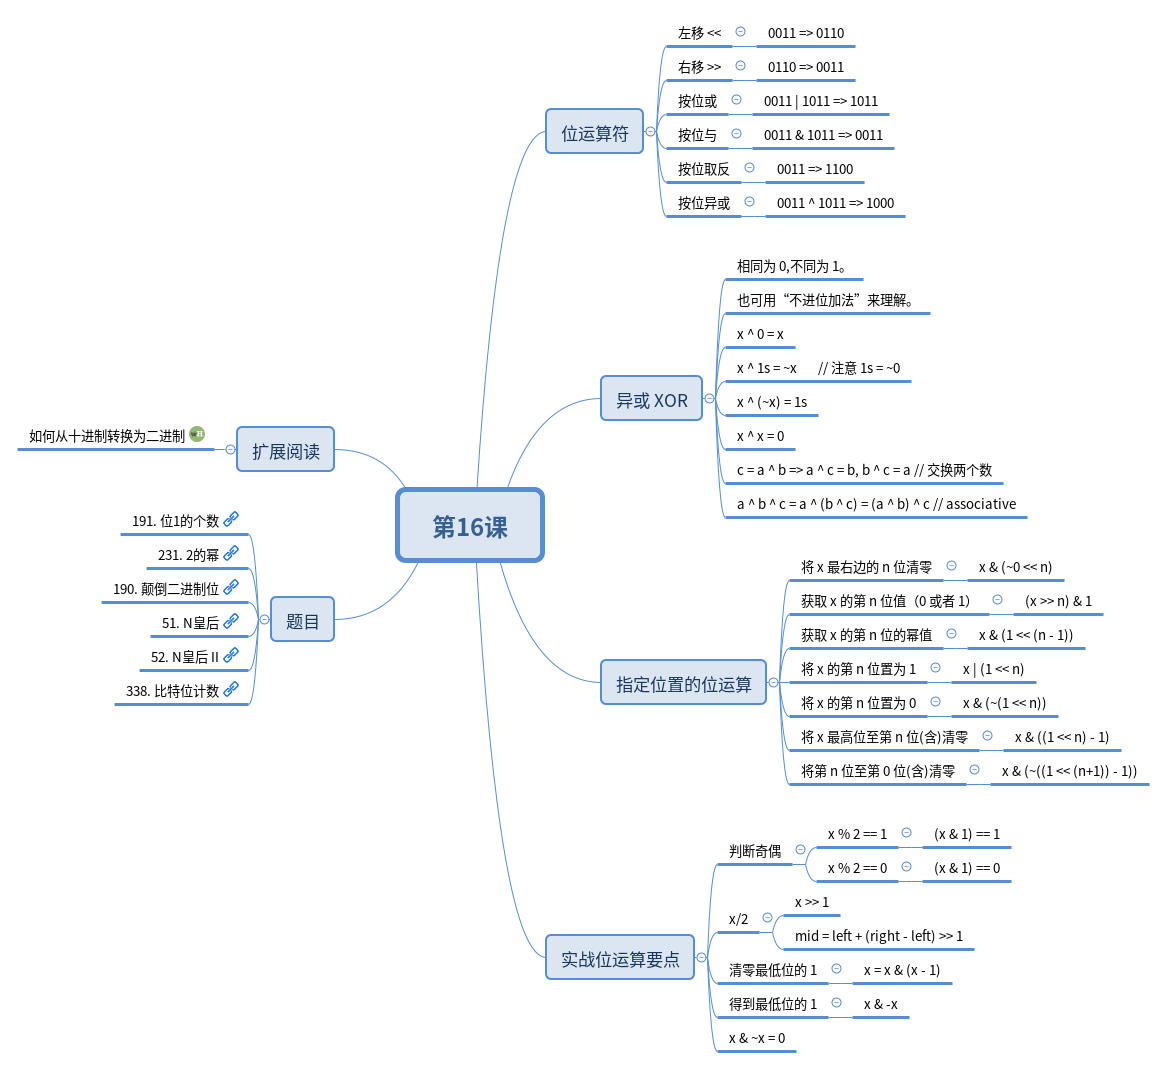
\includegraphics[width=160mm,height=150mm]{images/camp/第16课.png}

\subsubsection{题目}

\begin{itemize}
  \item \hyperref[leetcode:191]{191. 位1的个数}
  \item \hyperref[leetcode:231]{231. 2的幂}
  \item \hyperref[leetcode:190]{190. 颠倒二进制位}
  \item \hyperref[leetcode:51]{51. N皇后}
  \item \hyperref[leetcode:52]{52. N皇后 II}
  \item \hyperref[leetcode:338]{338. 比特位计数}
\end{itemize}

\subsubsection{扩展阅读}

\href{https://zh.wikihow.com/%E4%BB%8E%E5%8D%81%E8%BF%9B%E5%88%B6%E8%BD%AC%E6%8D%A2%E4%B8%BA%E4%BA%8C%E8%BF%9B%E5%88%B6}{如何从十进制转换为二进制}
